%---------change this for every latex homework
\def\yourid{rtg5xkh}
\def\collabs{ra9ha}
\def\sources{Cormen, et al, Introduction to Algorithms.}
% -----------------------------------------------------
\def\duedate{Friday, March 18, 2022 at 11:30 pm }
\def\duelocation{via Gradescope}
\def\htype{Basic}
\def\hunit{B}
\def\hnumber{2}
\def\course{{cs4102 - algorithms - spring 2022}}%------
%-------------------------------------
%-------------------------------------

\documentclass[10pt]{article}
\usepackage[colorlinks,urlcolor=blue]{hyperref}
\usepackage[osf]{mathpazo}
\usepackage{amsmath,amsfonts,graphicx}
\usepackage{latexsym}
\usepackage[top=1in,bottom=1.4in,left=1.25in,right=1.25in,centering,letterpaper]{geometry}
\usepackage{color}
\definecolor{mdb}{rgb}{0.1,0.6,0.4} 
\definecolor{cit}{rgb}{0.05,0.2,0.45} 
\pagestyle{myheadings}
\markboth{\yourid}{\yourid}
\usepackage{clrscode}
\usepackage{listings}

\newenvironment{proof}{\par\noindent{\it Proof.}\hspace*{1em}}{$\Box$\bigskip}
\newcommand{\handout}{
   \renewcommand{\thepage}{Unit \hunit: \htype~Homework \hnumber~-~\arabic{page}}
   \noindent
   \begin{center}
      \vbox{
    \hbox to \columnwidth {\sc{\course} \hfill}
    \vspace{-2mm}
       \hbox to \columnwidth {\sc due \MakeLowercase{\duedate} \duelocation\hfill {\Huge\color{mdb}\hunit\hnumber{\Large\MakeLowercase{\htype}}(\yourid)}}
      }
   \end{center}
   \vspace*{1mm}
   \hrule
   \vspace*{1mm}
    {\footnotesize \textbf{Collaboration Policy:} You are encouraged to collaborate with up to 3 other students, but all work submitted must be your own {\em independently} written solution. List the computing ids of all of your collaborators in the \texttt{collabs} command at the top of the tex file. Do not share written notes, documents (including Google docs, Overleaf docs, discussion notes, PDFs), or code.  Do not seek published or online solutions for any assignments. If you use any published or online resources (which may not include solutions) when completing this assignment, be sure to cite by naming the book etc.\ or listing a website's URL. Do not submit a solution that you are unable to explain orally to a member of the course staff. Any solutions that share similar text/code will be considered in breach of this policy. Please refer to the syllabus for a complete description of the collaboration policy.
   \vspace*{1mm}
    \hrule
    \vspace*{2mm}
    \noindent
    \textbf{Collaborators}: \collabs\\
    \textbf{Sources}: \sources}
    \vspace*{2mm}
    \hrule
    \vskip 2em
}

\newcommand{\solution}[1]{\color{blue}\hfill\break\noindent\textbf{Solution:} #1\color{black}}
\newcommand{\altsolution}[1]{\color{blue}\hfill\break\noindent\textbf{Solution (Alternative):} #1\color{black}}

%\newcommand{\solution}[1]{}
%\newcommand{\altsolution}[1]{}

\newcommand{\bit}[1]{\{0,1\}^{ #1 }}
%\dontprintsemicolon
%\linesnumbered
\newtheorem{problem}{\sc\color{cit}problem}
\newtheorem{practice}{\sc\color{cit}practice}
\newtheorem{lemma}{Lemma}
\newtheorem{definition}{Definition}
\newtheorem{theorem}{Theorem}

\newcommand{\Z}{\mathbb{Z}} % This might be useful for Integers!

\begin{document}
\thispagestyle{empty}
\handout

%----Begin your modifications here


%--- Problem 1 ------------------------------------------------------------------------------
\begin{problem} DFS and Topological Sort \end{problem}

\begin{enumerate}   

\item Run DFS on the following graph. List start and finish times (beginning at $t=1$) for each node in the table shown below the image of the graph. Note: For this problem, by "start" we mean the discovery time, and by "end" we mean finish times.) Use $V_1$ as your start node. \emph{To help us grade this more easily, when multiple nodes can be searched, always search neighboring nodes in increasing order (e.g., if $V_2$ and $V_3$ are both adjacent to the current node, search $V_2$ first)}.

\begin{center}
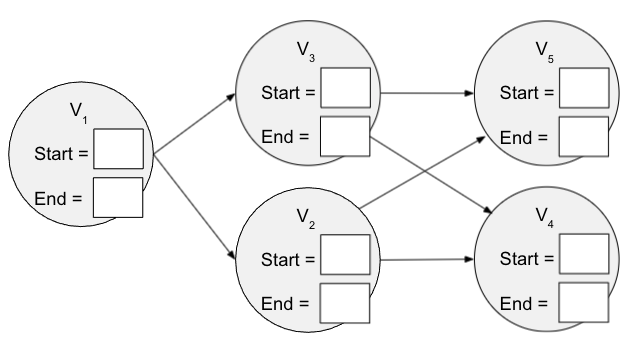
\includegraphics[scale=0.5]{graph_DFS}

%% Students: replace the ?'s in the table below with numbers
{\large
\begin{tabular}{|r|c|c|c|c|c|}
\hline \bf Vertex & $V_1$ & $V_2$ & $V_3$ & $V_4$ & $V_5$ \\
\hline \bf Start  & 1 & 2 & 8 & 3 & 5 \\
\hline \bf End    & 10 & 7 & 9 & 4 & 6 \\
\hline
\end{tabular}
}
\end{center}

\solution{
    See table.
}

\item Using your answer above, give the specific \emph{Topological Ordering} that would be produced by the \emph{DFS-based} algorithm we discussed in class.

\solution{
    $V_1$, $V_3$, $V_2$, $V_5$, $V_4$ \\
    (reverse order of finish times)
}

\end{enumerate}   

\pagebreak

%--- Problem 2 ------------------------------------------------------------------------------
\begin{problem} True or False. (You don't have to explain this in your submission, but you should understand the reason behind your answer.)  \end{problem}

\begin{enumerate}
\renewcommand{\theenumi}{\Alph{enumi}}

    \item  If you use DFS to find a topological sorting on a directed graph, the last vertex discovered in the search could legally be the last vertex in the sorted ordering of the vertices.
    \solution{
    True
    % consider a digraph with only 2 vertices, v1 and v2, and one edge from v1 to v2. Starting at v1, v2 will be the last vertex that's discovered and it will also be the last vertex in the topological sort.
    }
    
    \item For the disjoint set data structure we studied, if we had a $\Theta(\log n)$ implementation of \emph{find-set()}, then the order class for the time-complexity of \emph{union(i,j)} would be improved (i.e., better than the result we learned).
    \solution{
    True
    % union depends on find
    }
    
    \item Both path-compression and union-by-rank try to improve the cost of future calls to \emph{find-set()} by making the trees representing a set shorter without changing the set membership for the items in that set.
    \solution{
    True
    % 
    }
    
\end{enumerate}

%--- Problem 3 ------------------------------------------------------------------------------
\begin{problem} Kruskal's Runtime \end{problem}
What is the runtime of Kruskal’s algorithm if find() and union() are $\Theta(1)$ time?
\solution{
    Part of Kruskal's runtime (Every edge from PQ removed once) can be given by $\Theta\left(E*\left( 2f(V) + u(V) \right) \right)$ Where $f(V)$ is the runtime of find() and $u(V)$ is the runtime of union(). Thus, if find() and union() are $\Theta(1)$, this part of Kruskal's can be simplified down to just  $\Theta(E)$, which is $\Theta(V^{2})$. The other part of Kruskal's (for each edge 2 set finds and 1 set union) is $\Theta(E * log(V))$, so adding these two together we would get an overall runtime of $\Theta(E * log(V))$.
}

%--- Problem 4 ------------------------------------------------------------------------------
\begin{problem} Strongly Connected Components \end{problem}

Your friend Kai wants to find a digraph's SCCs by initially creating $G_T$ and running DFS on that. In other words, he believes he might be able to \textit{first} do something with the the transpose graph as the first step for finding the SCCs. (The algorithm we gave you first did something with $G$ and not with $G_T$.) \\
Do you think it's possible for Kai to make this approach work? If not, describe a counter-example or explain why this will fail. \\
If it is possible, explain the steps Kai's algorithm would have to do to complete the algorithm, and briefly say why this approach can lead to a correct solution.
\solution{
    Yes. He could do the same thing that the original algorithm did, however by taking the times from $G_T$ first, and them performing step 3 of CLRS's algorithm (Calling DFS-sweep($G_T$) with recursive calls on nodes in the order of decreasing finish times determined from G's DFS-sweep). This step would instead call DFS-sweep on $G$ based on times determined from $G_T$, so the calls to DFS-visit would still be in the correct order. Thus the result would still be the correct trees. These trees would still have their edges reversed, however we are only concerned about which vertices are members of which SCCs in this problem, and that part would remain the same. By reversing the steps and working with the different times, he would still be able to find the same SCCs, because taking the transpose graph does not create or remove any cycles from a digraph. 
}

\newpage 
%--- Problem 5 ------------------------------------------------------------------------------
\begin{problem} Executing Kruskal's MST Algorithm \end{problem}
Run Kruskal's algorithm on the graph below. List the order in which the edges are added to the MST, referring to the edges by their provided labels. \\
(\emph{Consider how your answer would change if E1 had weight 12.  However, you don't need to provide an answer to us for this part.})

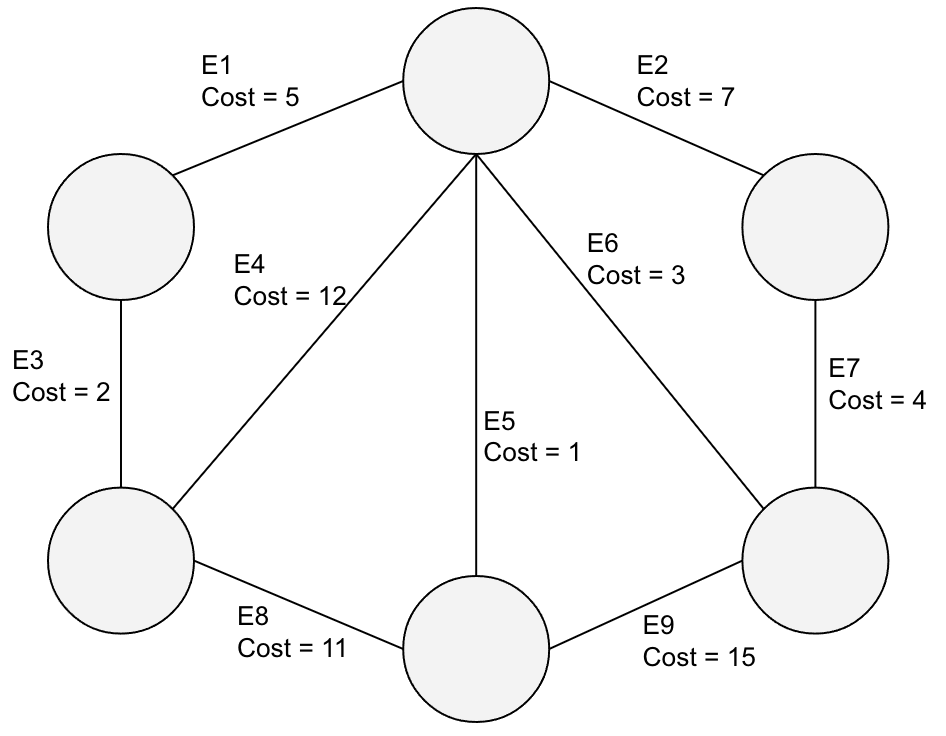
\includegraphics[scale=0.4]{graph_MST1}

Your answer (list of edges in order):
\solution{
    E5, E3, E6, E7, E1
}

%--- Problem 6 ------------------------------------------------------------------------------
\begin{problem} Difference between Prim's MST and Dijkstra's SP \end{problem}
In a few sentences, summarize the relatively small differences in the code for Prim's MST algorithm and Dijkstra's SP algorithm.
\solution{
    One key difference is that Dijkstra's must account for the distance to the current vertex when calculating the distance to a new vertex. Dijkstra's does this by adding the previous distance to the distance from the current vertex to the next and adding that to the Queue, while Prim's simply adds the distance from the current vertex to the next to the PQ. Similarly, when checking a fringe vertex, Dijkstra's must compare the entire distances to the vertex from the start vertex, while Prim's can simply compare the weights to the vertices. 
}

%--- Problem 7 ------------------------------------------------------------------------------
\begin{problem} True or False. (You don't have to explain this in your submission, but you should understand the reason behind your answer.)  \end{problem}

\begin{enumerate}
\renewcommand{\theenumi}{\Alph{enumi}}

\item An \emph{indirect heap} makes \emph{find()} and \emph{decreaseKey()} faster (among others), but \emph{insert()\/} becomes asymptotically slower because the indices in the indirect heap must be updated while percolating value up towards the root of the heap.
\solution{
    False
    % insert might be slightly slower by a constant, but it's not asymptotically slower
}

\item If all edges in an undirected connected graph have the same edge-weight value $k$, you can use either BFS or Dijkstra's algorithm to find the shortest path from $s$ to any other node $t$, but one will be more efficient than the other.
\solution{
    True
    % BFS will be faster
}

\item In the proof for the correctness of Dijkstra's algorithm, we learned that the proof fails if edges can have weight $0$ because this would mean that another edge could have been chosen to another fringe vertex that has a smaller distance than the fringe vertex chosen by Dijkstra's.
\solution{
    False
    % Even if edge weights could be 0 it would still work fine, the weights just can't be negative
}

\end{enumerate}

  

\begin{problem} Gradescope Submission \end{problem}
Submit a version of this \verb|.tex| file to Gradescope with your solutions added, along with the compiled PDF.  You should only submit your \verb|.pdf| and \verb|.tex| files.

\end{document}

